% !TeX root = ../main.tex

\section{Introduction}
\frame{\sectionpage}

\begin{frame}{Social Distancing under Pandemic}
  \begin{itemize}
    \item Social distancing measures
    \begin{columns}[c]  %开始进入分栏环境,居中设置
      \column{6cm}  %第一栏(左栏)宽度为5cm
      \begin{figure}[ht]
        \centering
        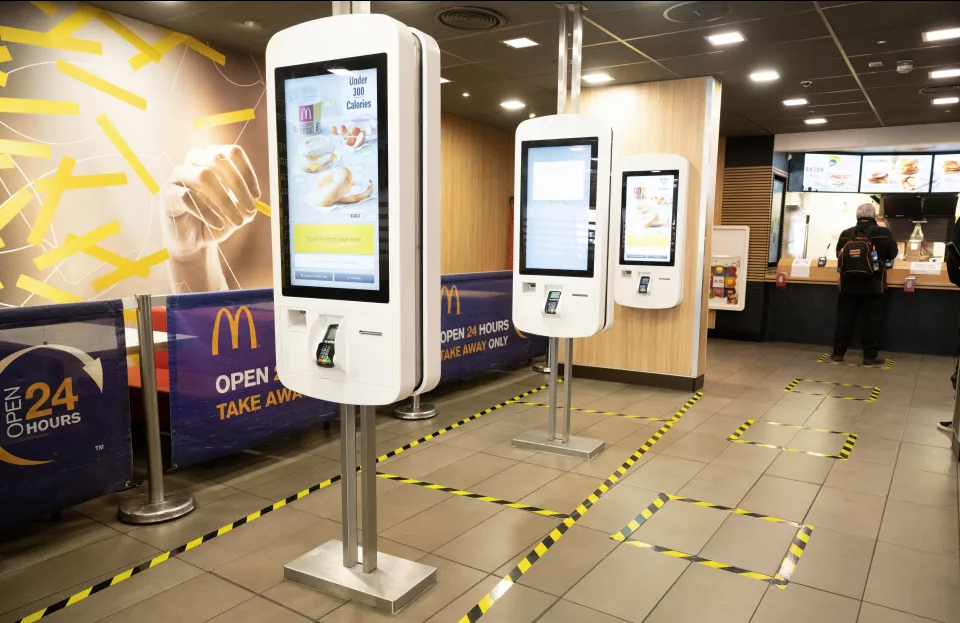
\includegraphics[width = 0.7\textwidth]{./images/McDonald.png}
        % \caption{Problem Conversion with One Seat as Social Distancing}
      \end{figure}
      \column{4cm}
      \scriptsize
      \begin{figure}[ht]
        \centering
        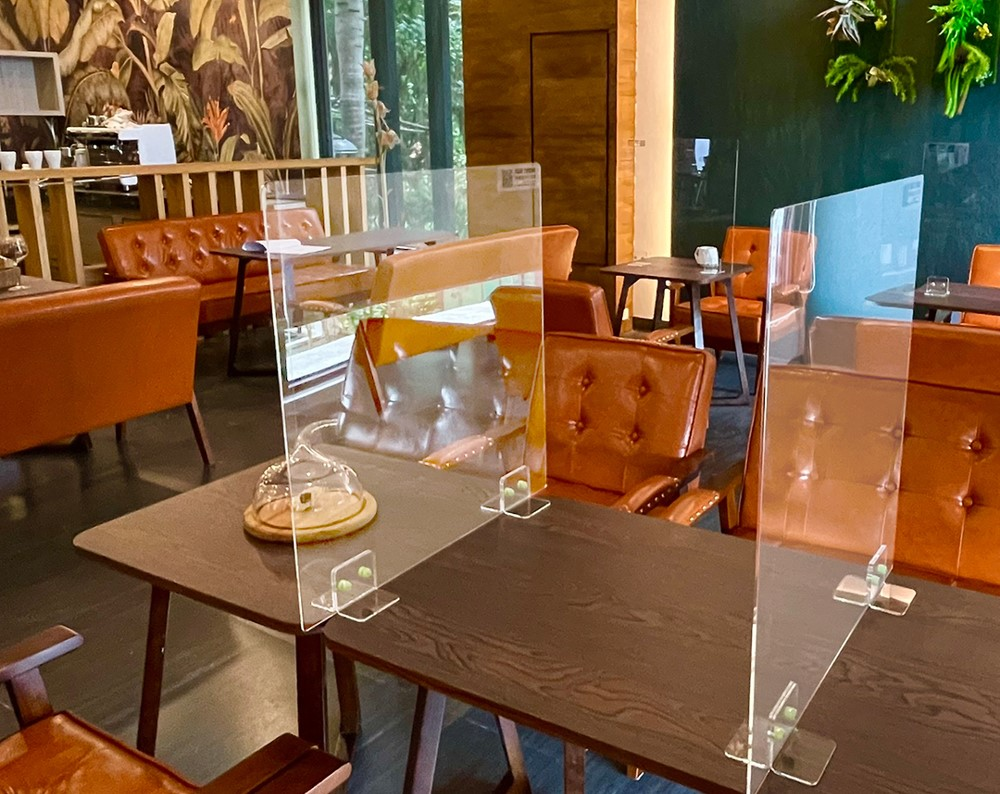
\includegraphics[width=0.9\textwidth,height=0.7\textwidth]{./images/res2.jpg}
        % \caption{Problem Conversion with One Seat as Social Distancing}
      \end{figure}
      \end{columns} 

      \begin{columns}[c]  %开始进入分栏环境,居中设置
        \column{5.5cm}  %第一栏(左栏)宽度为5cm
        \begin{figure}[ht]
          \centering
          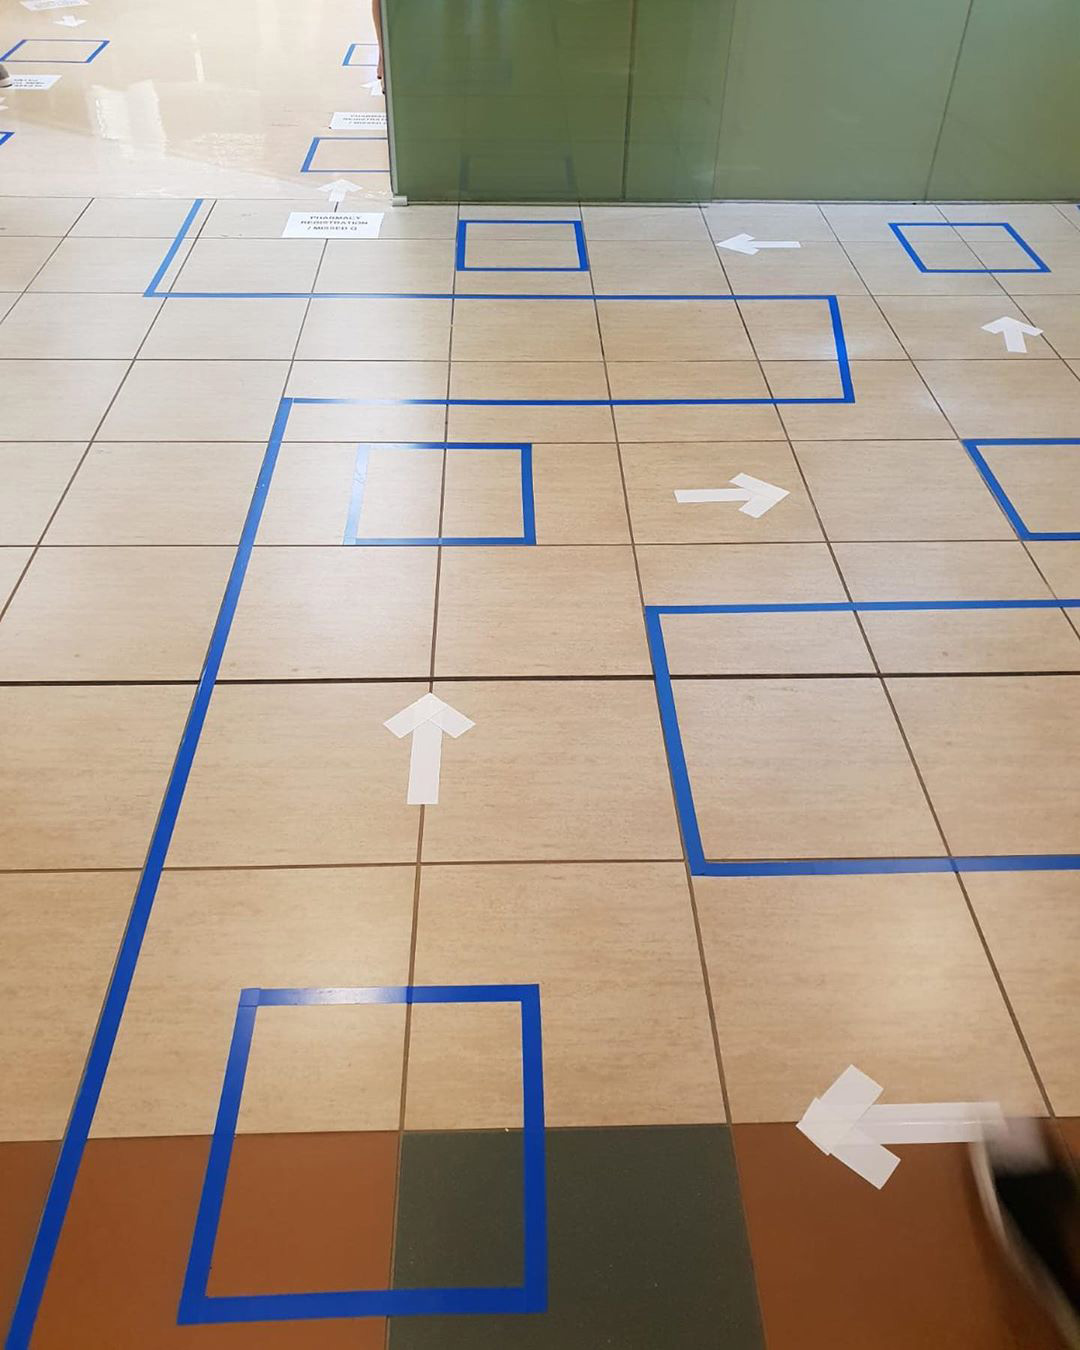
\includegraphics[width = 0.7\textwidth, height=0.5\textwidth]{./images/social_distancie_tape.jpg}
        \end{figure}
        \column{4.5cm}
        \scriptsize
        \begin{figure}[ht]
          \centering
          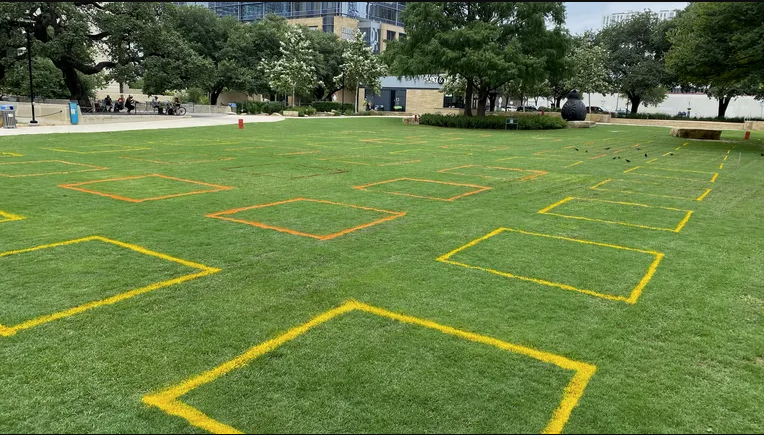
\includegraphics[width = 0.9\textwidth]{./images/socail_park.png}
        \end{figure}
        \end{columns} 
  \end{itemize}
  \end{frame}


  \begin{frame}{Social Distancing under Pandemic}
    \begin{itemize}
      \item Social distancing in seating areas
      \begin{columns}[c]  %开始进入分栏环境,居中设置
        \column{5cm}  %第一栏(左栏)宽度为5cm
        \begin{figure}[ht]
          \centering
          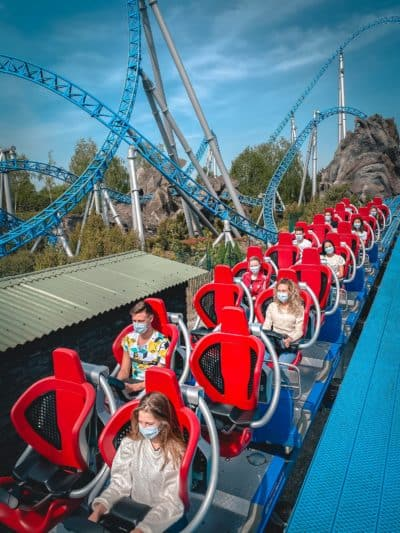
\includegraphics[width = 0.8\textwidth, height=0.6\textwidth]{./images/park_social_distancing.jpg}

        \end{figure}
        \column{5cm}
        \scriptsize
        \begin{figure}[ht]
          \centering
          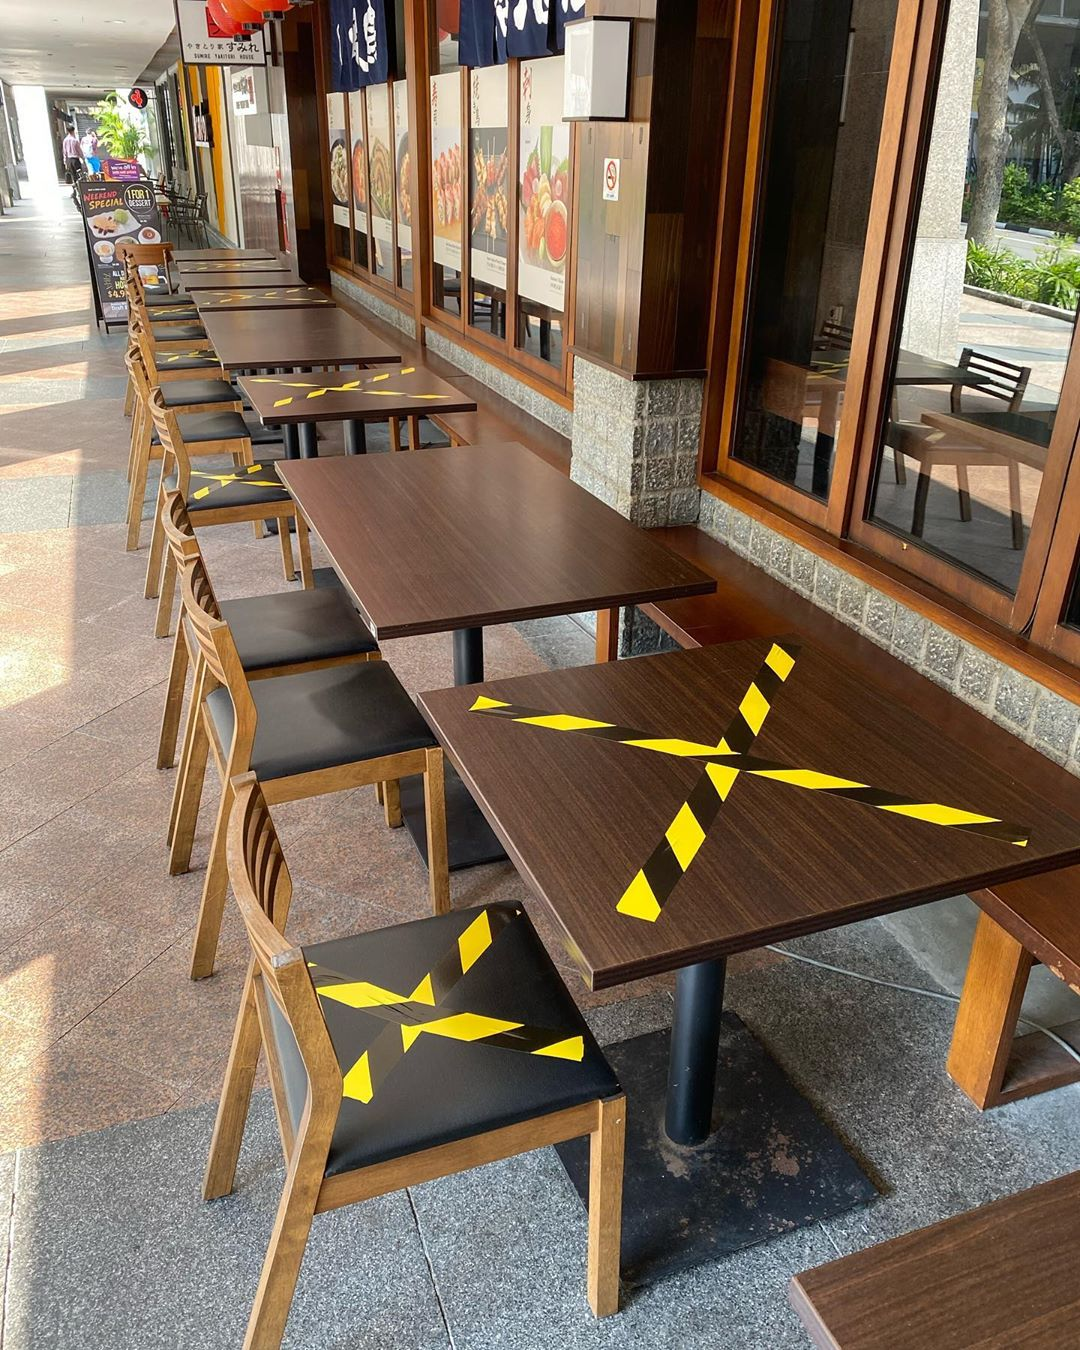
\includegraphics[width=0.8\textwidth,height=0.6\textwidth]{./images/tape_measures.jpg}
        \end{figure}

        \end{columns} 
        
        \begin{columns}[c]  %开始进入分栏环境,居中设置
          \column{5cm}  %第一栏(左栏)宽度为5cm
          \begin{figure}[ht]
            \centering
            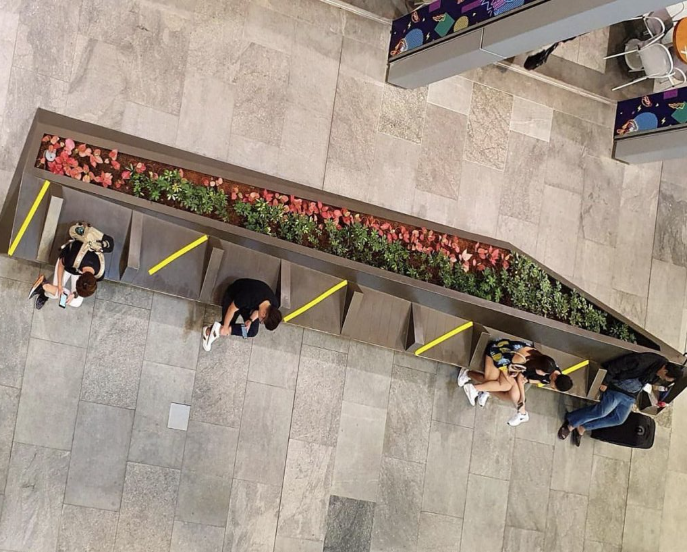
\includegraphics[width = 0.8\textwidth]{./images/seat_sc.png}
          \end{figure}
          \column{5cm}
          \scriptsize
          \begin{figure}[ht]
            \centering
            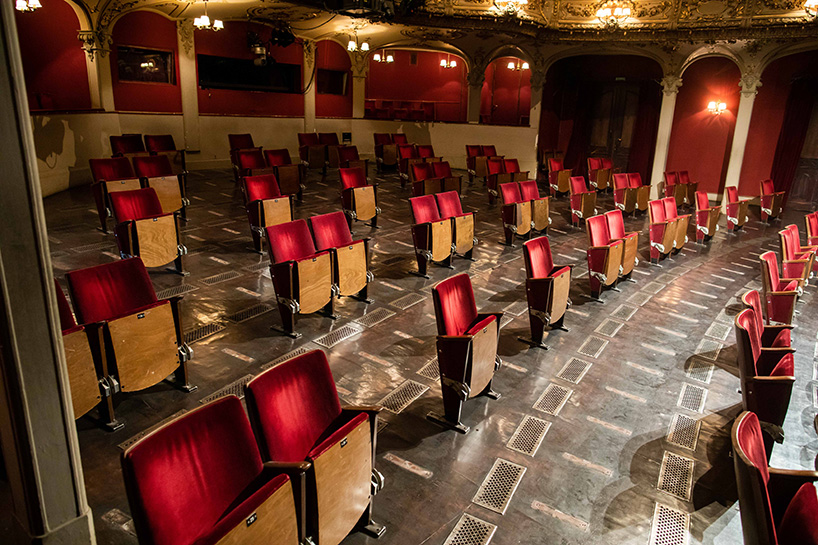
\includegraphics[width = 0.9\textwidth]{./images/cinema.jpg}
          \end{figure}
          \end{columns} 
    \end{itemize}
    \end{frame}

    \begin{frame}{Seat Planning and Seat Assignment}
      Social distancing requirement: 
      
      \begin{itemize}
        \item[-] The size of a group is confined.
        \item[-] People in the same group sit together.
        \item[-] Different groups should keep distance.
      \end{itemize}
      
      \vspace{0.5cm}

      % \begin{figure}[ht]
      %   \centering
      %   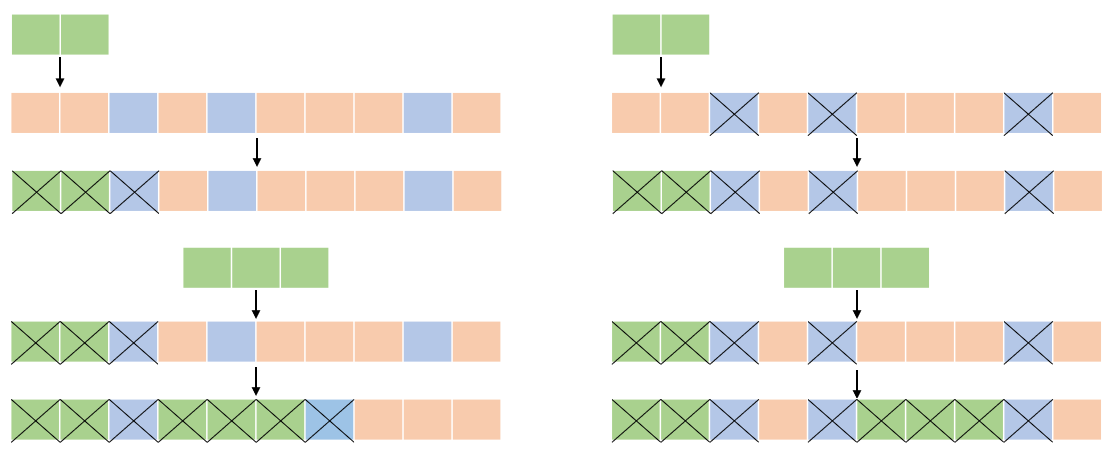
\includegraphics[width = 0.8\textwidth]{./images/assignment.png}
      % \end{figure}
      \begin{columns}
        \column{5cm}  %第一栏(左栏)宽度为5cm
        Seat planning: 
          \begin{figure}[ht]
            \centering
            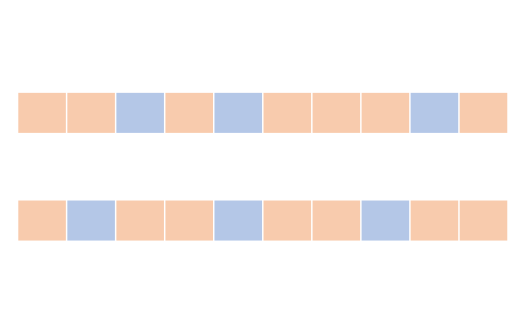
\includegraphics[width = 0.8\textwidth]{./images/seat_planning1.png}
          \end{figure}
          \column{5cm}
        Seat assignment:
          \scriptsize
          \begin{figure}[ht]
            \centering
            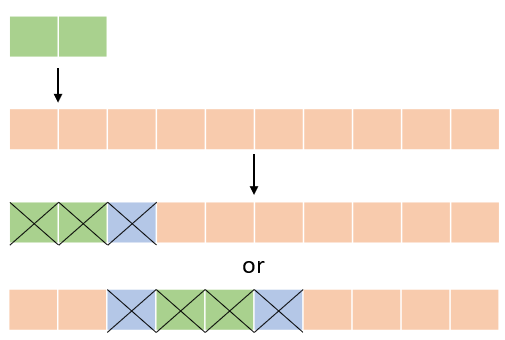
\includegraphics[width = 0.8\textwidth]{./images/seat_assignment1.png}
          \end{figure}
      \end{columns}
    \end{frame}
    

    \begin{frame}{Overview}
      \begin{itemize}
        \item Seat planning
        \vspace*{0.2cm}
        \begin{itemize}
          \item {\color{red}Deterministic demand}: make the seat planning with the known specific demand for groups.
          \item {\color{red} \textbf{Stochastic demand}}: make the seat planning with the known demand distribution before the realization of demand.
        \end{itemize}
        
        \item Seat assignment with dynamic demand
        
        \begin{itemize}
          \vspace*{0.2cm}
          \item Assign seats to each group under {\color{red}flexible} seat planning.
          \vspace*{0.2cm}
            \item[-] {\color{red} \textbf{Real-time seat assignment}}
            
            \vspace*{0.2cm}

            \item[-] Accept or reject each group after its realization, but assign them later.
          \vspace*{0.2cm}
          \item Assign seats to each group under {\color{red}fixed} seat planning.
        \end{itemize}
      \end{itemize}
    \end{frame}

    \begin{frame}{Contributions}
      \begin{itemize}
        \item  Seat planning:
        \vspace{0.2cm}

        \begin{itemize}
          \item New model and technique for stochastic demand
          \vspace{0.2cm}

          \item Provide seat planning as a guidance for seat assignment 
        \end{itemize}
        
        \vspace{0.8cm}
        
        \item Seat assignment:
        \vspace{0.2cm}

        \begin{itemize}
          \item New model for seat assignment problem
          \vspace{0.2cm}

          \item Provide practical solution and insights
        \end{itemize}
      
      \end{itemize}  

    \end{frame}